%
%  wl_hh_benford.tex
%
%  Created by Drew Conway on 2011-02-21
% 
%
\documentclass[xcolor=dvipsnames, 9pt]{beamer}

\newenvironment{code}{\begin{semiverbatim} \begin{footnotesize}}
{\end{footnotesize}\end{semiverbatim}}

% Running Headers and footers
%\usepackage{fancyhdr}

% Multipart figures
%\usepackage{subfigure}

\usepackage{graphicx}
\usepackage{amssymb}
\usepackage{amsfonts}
\usepackage{amsmath}
\usepackage{hyperref}
\usepackage{natbib}
\usepackage{color}
\usepackage{pdfsync}
\usepackage{chancery}
\usepackage{movie15}
\usepackage{pgfpages}
\usepackage{fancyvrb}
\usepackage{colortbl}
\usepackage{wasysym}

% \definecolor{white}{rgb}{255,255,255}
% \definecolor{darkred}{rgb}{0.5,0,0}
% \definecolor{darkgreen}{rgb}{0,0.5,0}
% \definecolor{lightblue}{rgb}{0,0,0.7}

% \hypersetup{colorlinks,
%   linkcolor=white,
%   filecolor=darkred,
%   urlcolor=lightblue,
%   citecolor=darkblue}

\usepackage{beamerthemesplit}
\usetheme{Copenhagen}
\usecolortheme[named=Blue]{structure} 
\setbeamertemplate{navigation symbols}{}
\setbeamertemplate{itemize items}[triangle]
\setbeamertemplate{enumerate items}[default]
%\setbeameroption{show notes on second screen}
%\logo{\includegraphics[width = 2cm]{nyulogo.png}}

\newcommand{\R}{\mathbb{R}}
\renewcommand{\d}{\mathsf{d}}
\newcommand{\dd}{\partial}
\newcommand{\E}{\mathsf{E}}
\newcommand{\bb}{\mathbf}

\title{Citizen Data-Driven Journalism\\The WikiLeaks Afghanistan War Logs}
\author{Drew Conway, Mike Dewar \& John Myles White}
\date{March 9, 2011}

\begin{document}
    
\ifpdf
\DeclareGraphicsExtensions{.pdf, .jpg, .tif}
\else
\DeclareGraphicsExtensions{.eps, .jpg}
\fi
% Set graphics path
\graphicspath{{images/}}

\begin{frame}[plain]
  \titlepage  
\end{frame}



\section{Introduction}

\begin{frame}
	\frametitle{Wikileaks}
	\begin{center}
    
\includegraphics[height=0.8\textheight]{wikileaks_eggtimer.png}
    \end{center}
\end{frame}

\begin{frame}
    \frametitle{Data Journalism}
    \begin{center}
    
\includegraphics[width=0.8\textwidth]{guardian.png}
    \end{center}
\end{frame}

\begin{frame}
    \frametitle{Citizen Data Analysis}
    \begin{center}
    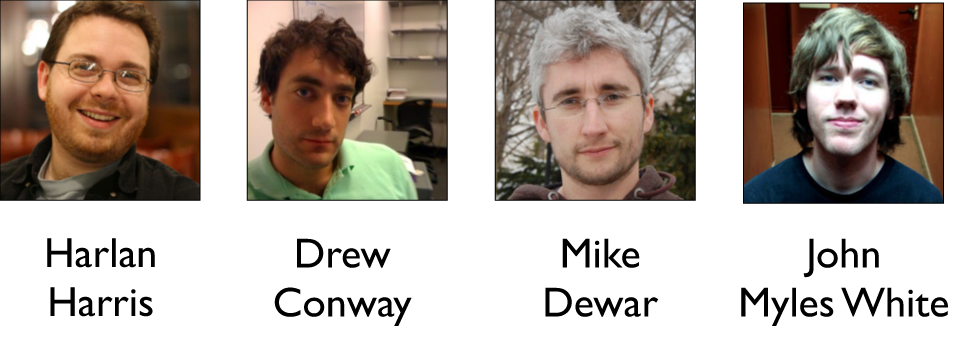
\includegraphics[width=\textwidth]{hackademics.png}
    \end{center}
\end{frame}

{
\setbeamertemplate{background canvas}{
\includegraphics 
	[width=\paperwidth,height=\paperheight]{hackabit.png}} 
\begin{frame}
    \frametitle{Hackabit}
\end{frame}
}

\begin{frame}
    \frametitle{A Taxonomy of Data Science}
    
    \begin{center}
        
        \begin{columns}[c] 
            \column{.5\textwidth}
            \begin{itemize}
                \item Obtain
                \item Scrub
                \item Explore
                \item Model
                \item iNterpret
            \end{itemize}
\column{.5\textwidth} 
\huge{O.S.E.M.N.}\\
        \vspace{1em}

\includegraphics[width=0.9\textwidth]{possum.png}
\end{columns}            
        
    \end{center}
\end{frame}

{
\setbeamertemplate{background canvas}{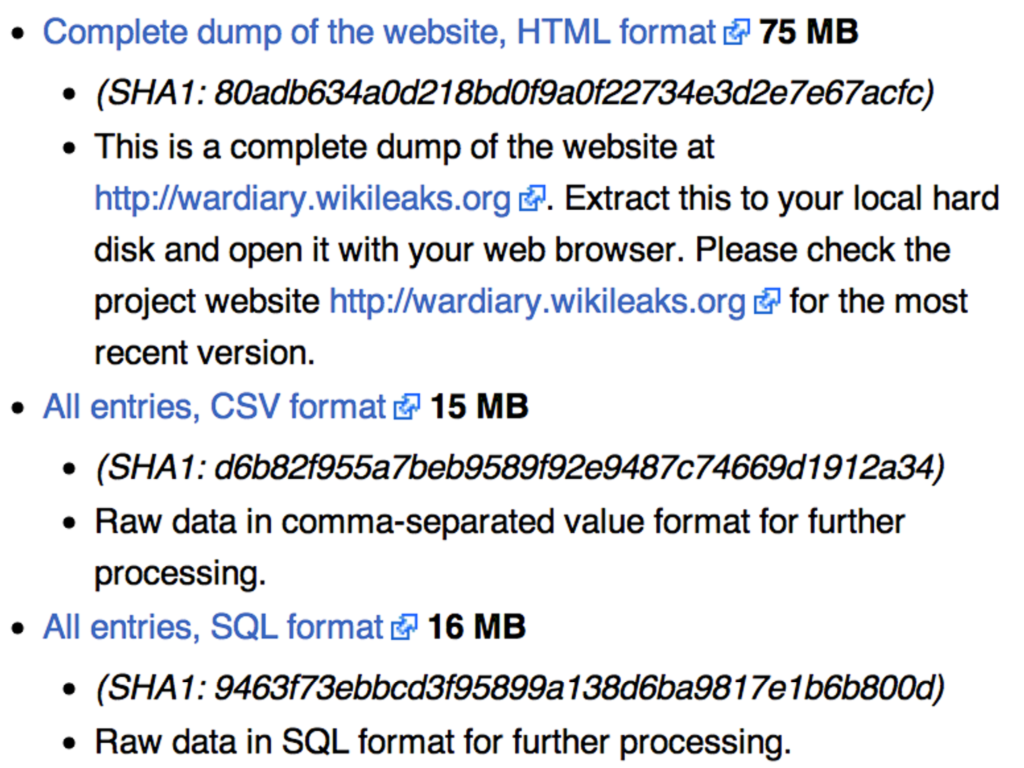
\includegraphics 
	[width=\paperwidth,height=\paperheight]{website.png}} 
\begin{frame}
    \frametitle{Obtain}
\end{frame}
}

\begin{frame}
    \frametitle{Scrub}
    \begin{center}
    
\includegraphics[width=0.5\textwidth]{pickaxe.png}
    \end{center}
\end{frame}

{
\setbeamertemplate{background canvas}{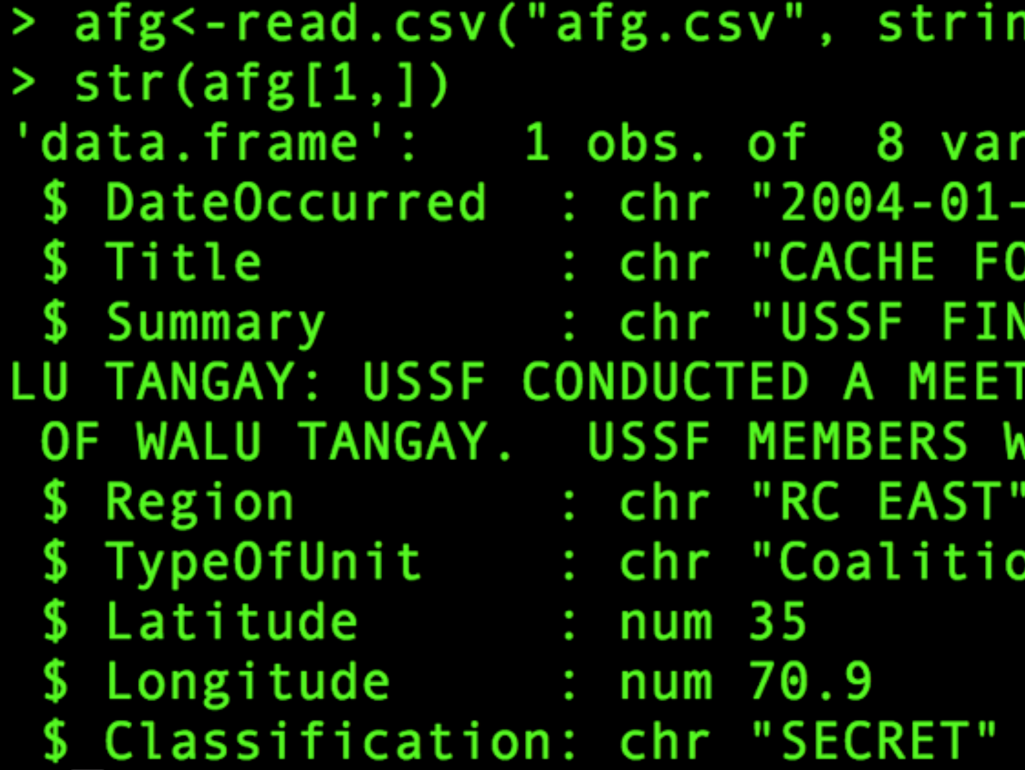
\includegraphics 
	[width=\paperwidth,height=\paperheight]{terminal.png}} 
\begin{frame}
    \frametitle{Explore}
\end{frame}
}

\begin{frame}
    \frametitle{Model}
    \begin{center}
    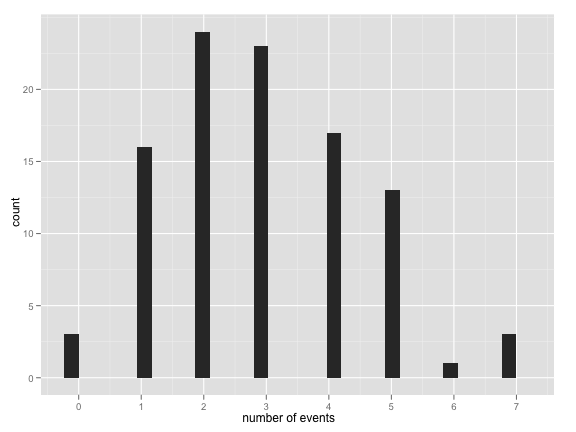
\includegraphics[width=0.9\textwidth]{histogram.png}
    \end{center}
\end{frame}

\begin{frame}
    \frametitle{Model}
    \begin{center}
    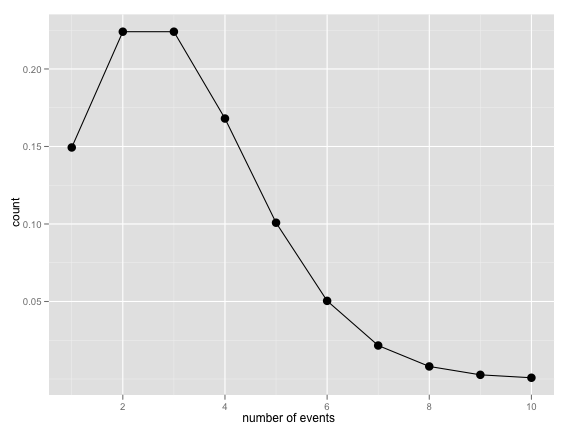
\includegraphics[width=0.9\textwidth]{distribution.png}
    \end{center}
\end{frame}

\begin{frame}
    \frametitle{Model}
    \begin{center}
    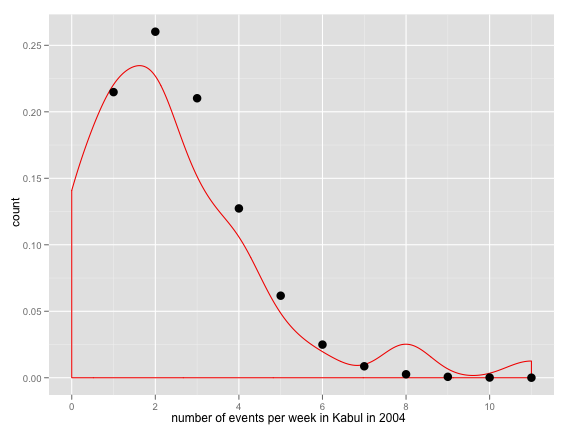
\includegraphics[width=0.9\textwidth]{density_estimate.png}
    \end{center}
\end{frame}

\begin{frame}
    \frametitle{iNterpret}
    \begin{center}
    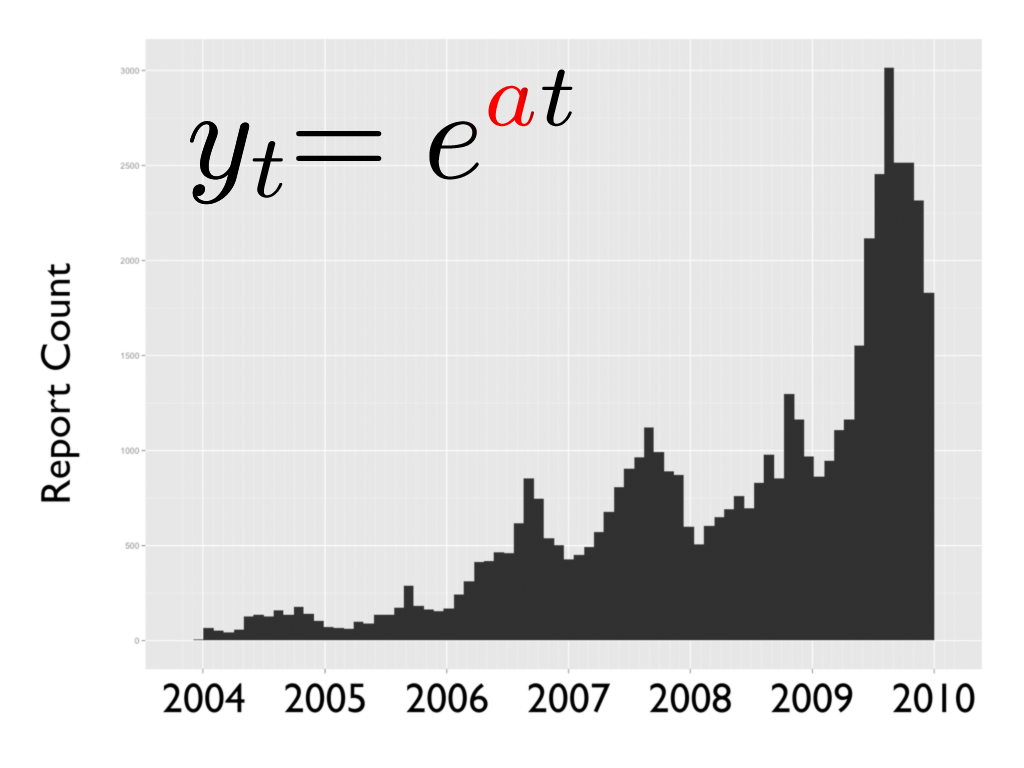
\includegraphics[width=0.9\textwidth]{time_course.png}
    \end{center}
\end{frame}

\section{Checking the data} % (fold)
\label{sec:checking_the_data}

\begin{frame}[fragile]
    \frametitle{Why is it important to check the data?}
    \uncover<2->{\begin{center}
        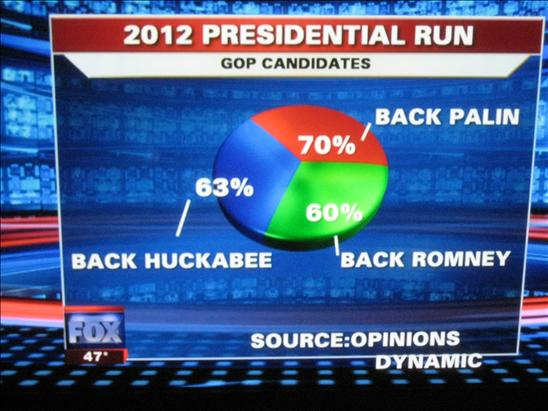
\includegraphics[width=9cm]{fox_news_pie_chart.png}
    \end{center}
    \tiny{\emph{Source}: \href{http://flowingdata.com/2009/11/26/fox-news-makes-the-best-pie-chart-ever/}{http://flowingdata.com/}}}
\end{frame}


\begin{frame}[fragile]
    \frametitle{Greater difficulty in the age of ``big data''}
        With crowd-sourced and dubiously disclosed data we have several issues
        \begin{itemize}
            \item Extremely difficult to vet---especially for non-journalists
            \item Data in ``raw'' form, high degree of variance 
            \item Motivation of sources unknown
        \end{itemize}
        \uncover<2->{\begin{block}{\emph{CJR} -- `The Challenge of Verifying Crowdsourced Information'}
            ``Even though the information from Twitter is not particularly reliable---and things are being retweeted so it’s kind of messy---the basic idea is if you crowdsource the information and put it on one map you can really see the clusters of incidents.  So even though one particular tweet is not that important, if you have similar reports from the media … you can see where the incidents are clustering.''\\
            \hfill{- Jaroslav Valuch, the project manager for Ushahidi Haiti}
        \end{block}}
        \uncover<3->{But...visual evidence can be deceiving
        \begin{itemize}
            \item Need a real test (statistical) to provide better evidence that data is reliable and not fraudulent
        \end{itemize}
        \tiny{Source: `\href{http://www.cjr.org/behind_the_news/the_challenge_of_verifying_cro.php}{The Challenge of Verifying Crowdsourced Information}},' see also: `\href{http://www.cjr.org/campaign_desk/how_wikileaks_outsourced_the_b.php?page=all}{How WikiLeaks Outsourced the Burden of Verification}'}}
\end{frame}

\begin{frame}[fragile]
    \frametitle{How to verify the data}
    First, are we trying to verify the information, or data itself?
    \begin{itemize}
        \item Former requires independent information and resources 
        \item Latter we can do statistically for free! $\smiley$
    \end{itemize}
    \uncover<2->{If simply verifying data as it exists, need a \textbf{data appropriate test}
    \begin{itemize}
        \item What do our data look like?
        \item What is the generating process?
    \end{itemize}}
    \uncover<3->{Journalists often deal with \textbf{discrete count data} wherein additional information has been coded into each event
    \begin{columns}
        \column{.65\textwidth}
            \begin{itemize}
                \item Election:  \# people voting for some candidate per-district
                \item Finance:   \# securities traded per-day
                \item Ushahidi:  \# incidents reported of some type
                \item WikiLeaks: \# SIGACTS per-region or geo-code
            \end{itemize}
        \column{.35\textwidth}
            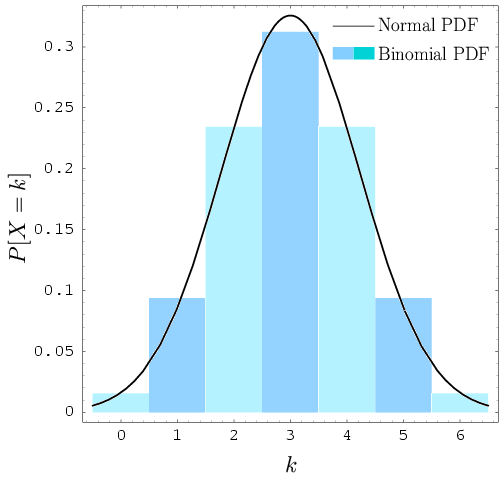
\includegraphics[width=3.2cm]{BinDistApprox_large.png}
    \end{columns}}
    \uncover<4->{We use \textbf{Benford's Law} to test that WikiLeaks data fits a \emph{natural data generating process} for count data}\\
    \uncover<4->{\tiny{Source: \url{http://en.wikipedia.org/wiki/Binomial_distribution}}}
\end{frame}


\begin{frame}[fragile]
    \frametitle{What is Benford's Law}
    \begin{block}{Benford's Law}
       Benford's law, also called the first-digit law, states that in lists of numbers from many (but not all) real-life sources of data, the leading digit is distributed in a specific, non-uniform way. According to this law, the first digit is 1 about 30\% of the time, and larger digits occur as the leading digit with lower and lower frequency, to the point where 9 as a first digit occurs less than 5\% of the time.\\
    \end{block}
    \begin{columns}
        \column{.4\textwidth}
            \uncover<2->{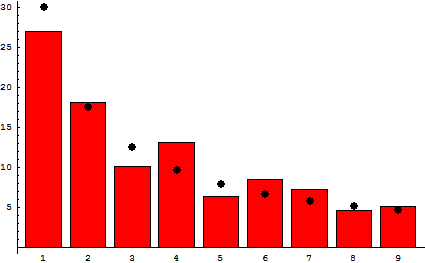
\includegraphics[width=5cm]{Benfords_law_illustrated_by_world's_countries_population.png}}\\
        \column{.6\textwidth}
            \begin{itemize}
                \uncover<2->{\item Distribution of first digits in the population of the 237 countries of the world (at left)}
                \uncover<3->{\item Detect check fraud (\href{http://www.journalofaccountancy.com/Issues/1999/May/nigrini}{\emph{Journal of Accountancy}})
                
                \item Election rigging in Iran (\href{http://www.fivethirtyeight.com/2009/06/statistical-evidence-does-not-prove.html}{FiveThirtyEight})}
            \end{itemize}
    \end{columns}
    \vspace{2mm}
    \uncover<4->{For the WikiLeaks, we will analyze the leading digits for \textbf{weekly counts of SIGACT reports} in the data
    \begin{itemize}
        \item This includes visual and statistical tests with Benford's Law
    \end{itemize}}
    \uncover<4->{\tiny{Source: \url{http://en.wikipedia.org/wiki/Benford's_law}}}
\end{frame}

\begin{frame}[fragile]
    \frametitle{Running the test}
    \begin{columns}
        \column{.8\textwidth}
            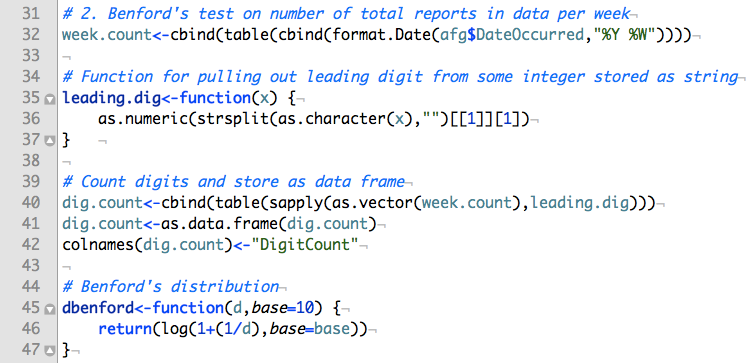
\includegraphics[width=9.2cm]{r_code1.png}
        \column{.2\textwidth}
            \only<2>{\alert{\textbf{\Huge{$\leftarrow$}}}} \\
            \vspace{8mm}
            \only<3>{\alert{\textbf{\Huge{$\leftarrow$}}}} % yo I can't compile if this \\ is left here!
            \vspace{1.5cm}
            \only<4>{\alert{\textbf{\Huge{$\leftarrow$}}}}
            \vspace{1.7cm}
    \end{columns}
    \vspace{1mm}
    \hline
    \begin{columns}
        \column{.33\textwidth}
            \begin{center}
                \uncover<2->{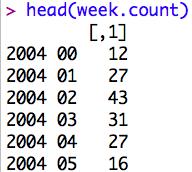
\includegraphics[width=2cm]{r_code2.png}}
            \end{center}
        \column{.33\textwidth}
            \begin{center}
                \uncover<2->{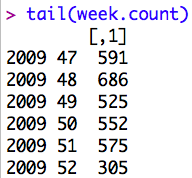
\includegraphics[width=2cm]{r_code2_5.png}}
            \end{center}
        \column{.33\textwidth}
            \begin{center}
                \uncover<4->{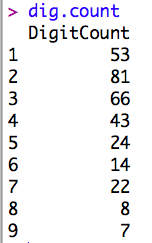
\includegraphics[width=1.7cm]{r_code3.png}}
            \end{center}
    \end{columns}
\end{frame}

\begin{frame}[fragile]
    \frametitle{Results 1 -- all of the data}
        \begin{columns}
            \column{.7\textwidth}
                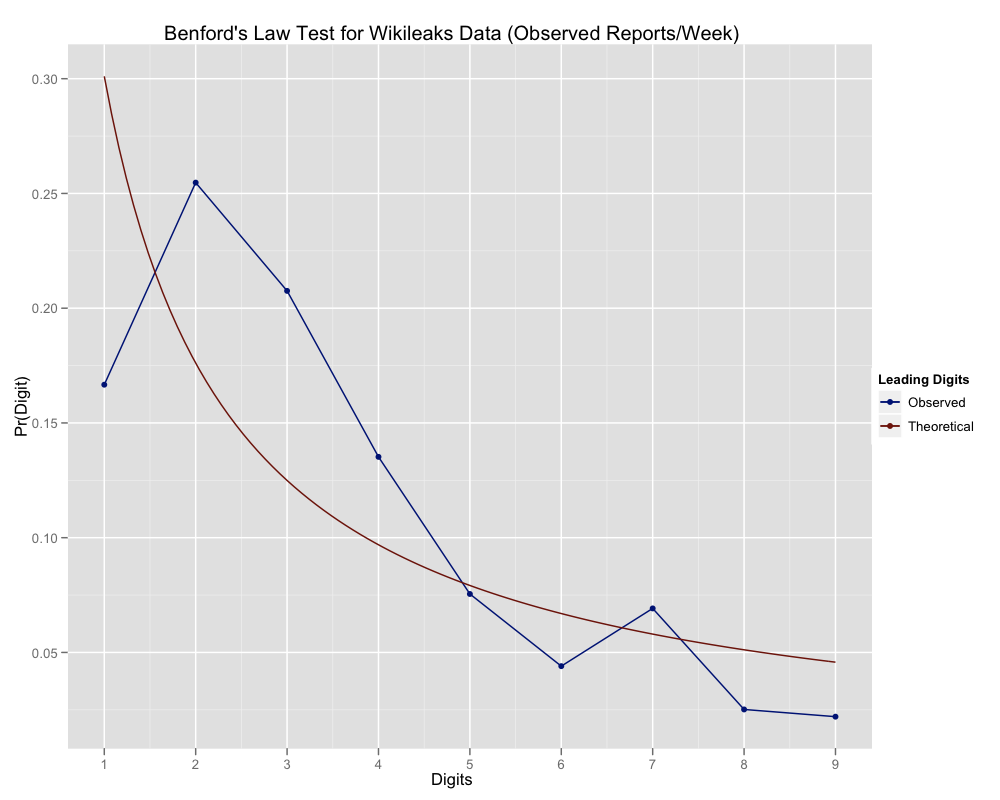
\includegraphics[width=8.5cm]{benford_all.png}
            \column{.3\textwidth}
            Chi-squared goodness of fit test
            \begin{itemize}
                \item $\chi^{2}=72$
                \item p-value=0.23
            \end{itemize}
            \vspace{3.3cm}
        \end{columns}
        \textbf{Cannot reject null} that data came from Benford-like data generating process}
\end{frame}

\begin{frame}[fragile]
    \frametitle{Results 2 -- by region}
    \begin{center}
        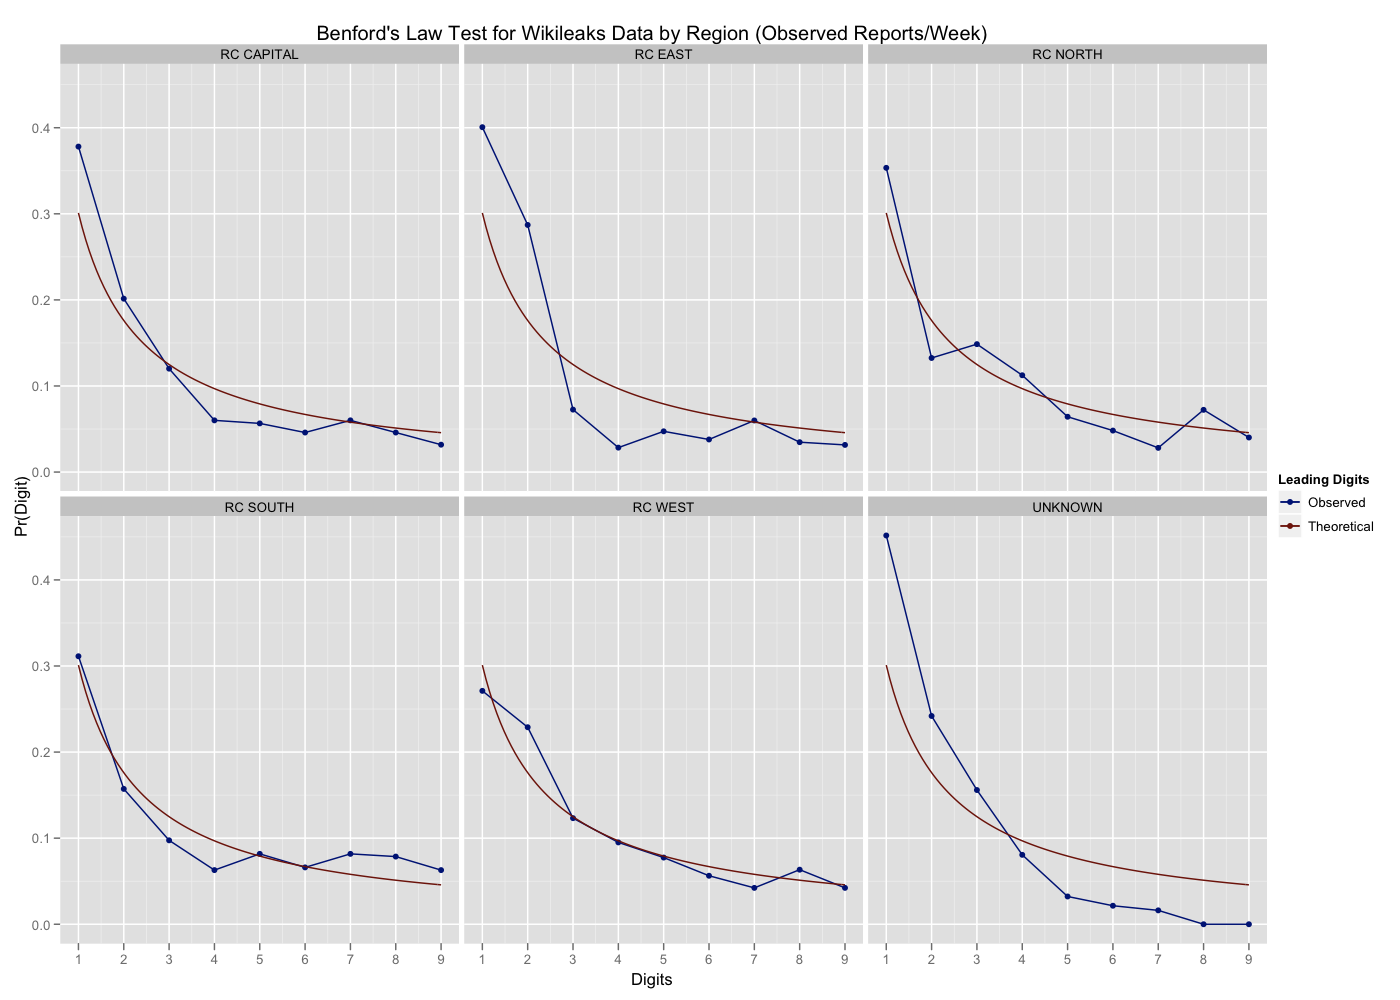
\includegraphics[width=10cm]{benford_region.png}
    \end{center}
\end{frame}

% section checking_the_data (end)


\end{document}
